\documentclass[12pt]{article}
\usepackage[utf8]{inputenc}
\usepackage{float}
\usepackage{amsmath}
\usepackage[tableaux]{prooftrees}
\renewcommand*\linenumberstyle[1]{(#1)}

\usepackage[hmargin=3cm,vmargin=6.0cm]{geometry}
\topmargin=-2cm
\addtolength{\textheight}{6.5cm}
\addtolength{\textwidth}{2.0cm}
\setlength{\oddsidemargin}{0.0cm}
\setlength{\evensidemargin}{0.0cm}
\usepackage{indentfirst}
\usepackage{amsfonts}
\usepackage{tikz}
\usepackage{qtree}
% \usepackage{pmatrix}

\begin{document}

\section*{Student Information}

Name: Kaan Karaçanta \\

ID: 2448546 \\


\section*{Part 1}

\subsection*{\text{a)}}

\paragraph*{Matrix A}

$$ A = 
\begin{bmatrix} 
        0 & 0 \\ 
        1 & 1 
    \end{bmatrix} $$

This matrix is not unitary because it cannot be inverted (determinant is 0), so it cannot be a quantum gate.

\paragraph*{Matrix B}

$$ B = 
\frac{1}{\sqrt{2}} \begin{bmatrix}
                        1 & 1 \\ 
                        1 & -1 
                    \end{bmatrix}
$$

This is the Hadamard gate. It creates a superposition of $|0⟩$ and $|1⟩$ when applied to a qubit. 

\paragraph*{Matrix C}

$$ C =
\begin{bmatrix}
    1 & 0 \\
    0 & -1
\end{bmatrix}
$$

This is a known quantum gate, the Pauli-Z (or Z) gate. It does not change the $|0⟩$ state, and for $|1⟩$ it gives $-|1⟩$.

\paragraph*{Matrix D}

$$ D =
\begin{bmatrix}
    1 & 1 \\
    1 & 1
\end{bmatrix}
$$

This matrix also does not describe a valid quantum gate because it is not unitary, and it cannot be inverted.

\paragraph*{Matrix E}

$$ E =
\begin{bmatrix}
    0 & 1 \\
    1 & 0
\end{bmatrix}
$$

This is also a known quantum gate, the Pauli-X (or X) gate. It swaps the amplitudes of the $|0⟩$ and $|1⟩$ states of a qubit.

\paragraph*{Matrix F}

$$ F = 
\begin{bmatrix}
    1 & 0 & 0 & 1 \\
    0 & 0 & 0 & 0 \\
    0 & 0 & 0 & 0 \\
    1 & 0 & 0 & 1
\end{bmatrix}
$$ 

This matrix is not a quantum gate as it does not satisfy the criteria for unitarity like A and D.

\paragraph*{Matrix G}

$$ G =
\begin{bmatrix}
    1 & 0 & 0 & 0 \\
    0 & 1 & 0 & 0 \\
    0 & 0 & 0 & 1 \\
    0 & 0 & 1 & 0
\end{bmatrix}
$$

This is a valid two-qubit quantum gate, the CNOT gate. It performs the NOT operation on the second qubit only when the first qubit is $|1⟩$.

\subsection*{\text{b)}}

Now, for the single qubit quantum gates (B, C, E), we can calculate the results with the inputs $|0⟩$, $|1⟩$, $|+⟩$, $|-⟩$ and for the 2-qubit gate (G), the inputs $|00⟩$, $|01⟩$, $|10⟩$, $|11⟩$. 

\paragraph*{B - Hadamard Gate}

$$ H(|0⟩) = \frac{1}{\sqrt{2}} \begin{bmatrix} 1 & 1 \\ 1 & -1 \end{bmatrix} \begin{bmatrix} 1 \\ 0 \end{bmatrix} = \frac{1}{\sqrt{2}} \begin{bmatrix} 1 \\ 1 \end{bmatrix} = \frac{1}{\sqrt{2}} (|0⟩ + |1⟩) = |+⟩ $$

$$ H(|1⟩) = \frac{1}{\sqrt{2}} \begin{bmatrix} 1 & 1 \\ 1 & -1 \end{bmatrix} \begin{bmatrix} 0 \\ 1 \end{bmatrix} = \frac{1}{\sqrt{2}} \begin{bmatrix} 1 \\ -1 \end{bmatrix} = \frac{1}{\sqrt{2}} (|0⟩ - |1⟩) = |-⟩ $$

$$ H(|+⟩) = \frac{1}{\sqrt{2}} \begin{bmatrix} 1 & 1 \\ 1 & -1 \end{bmatrix} \frac{1}{\sqrt{2}} \begin{bmatrix} 1 \\ 1 \end{bmatrix} = \frac{1}{2} \begin{bmatrix} 2 \\ 0 \end{bmatrix} = \begin{bmatrix} 1 \\ 0 \end{bmatrix} = |0⟩ $$

$$ H(|-⟩) = \frac{1}{\sqrt{2}} \begin{bmatrix} 1 & 1 \\ 1 & -1 \end{bmatrix} \frac{1}{\sqrt{2}} \begin{bmatrix} 1 \\ -1 \end{bmatrix} = \frac{1}{2} \begin{bmatrix} 0 \\ 2 \end{bmatrix} = \begin{bmatrix} 0 \\ 1 \end{bmatrix} = |1⟩ $$

\paragraph*{C - Pauli-Z Gate}

$$ Z(|0⟩) = \begin{bmatrix} 1 & 0 \\ 0 & -1 \end{bmatrix} \begin{bmatrix} 1 \\ 0 \end{bmatrix} = \begin{bmatrix} 1 \\ 0 \end{bmatrix} = |0⟩ $$

$$ Z(|1⟩) = \begin{bmatrix} 1 & 0 \\ 0 & -1 \end{bmatrix} \begin{bmatrix} 0 \\ 1 \end{bmatrix} = \begin{bmatrix} 0 \\ -1 \end{bmatrix} = -|1⟩ $$

$$ Z(|+⟩) = \begin{bmatrix} 1 & 0 \\ 0 & -1 \end{bmatrix} \frac{1}{\sqrt{2}} \begin{bmatrix} 1 \\ 1 \end{bmatrix} = \frac{1}{\sqrt{2}} \begin{bmatrix} 1 \\ -1 \end{bmatrix} = \frac{1}{\sqrt{2}} (|0⟩ - |1⟩) = |-⟩ $$

$$ Z(|-⟩) = \begin{bmatrix} 1 & 0 \\ 0 & -1 \end{bmatrix} \frac{1}{\sqrt{2}} \begin{bmatrix} 1 \\ -1 \end{bmatrix} = \frac{1}{\sqrt{2}} \begin{bmatrix} 1 \\ 1 \end{bmatrix} = \frac{1}{\sqrt{2}} (|0⟩ + |1⟩) = |+⟩ $$

\paragraph*{E - Pauli-X Gate}

$$ X(|0⟩) = \begin{bmatrix} 0 & 1 \\ 1 & 0 \end{bmatrix} \begin{bmatrix} 1 \\ 0 \end{bmatrix} = \begin{bmatrix} 0 \\ 1 \end{bmatrix} = |1⟩ $$

$$ X(|1⟩) = \begin{bmatrix} 0 & 1 \\ 1 & 0 \end{bmatrix} \begin{bmatrix} 0 \\ 1 \end{bmatrix} = \begin{bmatrix} 1 \\ 0 \end{bmatrix} = |0⟩ $$

$$ X(|+⟩) = \begin{bmatrix} 0 & 1 \\ 1 & 0 \end{bmatrix} \frac{1}{\sqrt{2}} \begin{bmatrix} 1 \\ 1 \end{bmatrix} = \frac{1}{\sqrt{2}} \begin{bmatrix} 1 \\ 1 \end{bmatrix} = \frac{1}{\sqrt{2}} (|0⟩ + |1⟩) = |+⟩ $$

$$ X(|-⟩) = \begin{bmatrix} 0 & 1 \\ 1 & 0 \end{bmatrix} \frac{1}{\sqrt{2}} \begin{bmatrix} 1 \\ -1 \end{bmatrix} = \frac{1}{\sqrt{2}} \begin{bmatrix} -1 \\ 1 \end{bmatrix} = \frac{1}{\sqrt{2}} (|0⟩ - |1⟩) = -|-⟩ $$

\paragraph*{G - CNOT Gate}

$$ CNOT(|00⟩) = \begin{bmatrix} 1 & 0 & 0 & 0 \\ 0 & 1 & 0 & 0 \\ 0 & 0 & 0 & 1 \\ 0 & 0 & 1 & 0 \end{bmatrix} \begin{bmatrix} 1 \\ 0 \\ 0 \\ 0 \end{bmatrix} = \begin{bmatrix} 1 \\ 0 \\ 0 \\ 0 \end{bmatrix} = |00⟩ $$

$$ CNOT(|01⟩) = \begin{bmatrix} 1 & 0 & 0 & 0 \\ 0 & 1 & 0 & 0 \\ 0 & 0 & 0 & 1 \\ 0 & 0 & 1 & 0 \end{bmatrix} \begin{bmatrix} 0 \\ 1 \\ 0 \\ 0 \end{bmatrix} = \begin{bmatrix} 0 \\ 1 \\ 0 \\ 0 \end{bmatrix} = |01⟩ $$

$$ CNOT(|10⟩) = \begin{bmatrix} 1 & 0 & 0 & 0 \\ 0 & 1 & 0 & 0 \\ 0 & 0 & 0 & 1 \\ 0 & 0 & 1 & 0 \end{bmatrix} \begin{bmatrix} 0 \\ 0 \\ 1 \\ 0 \end{bmatrix} = \begin{bmatrix} 0 \\ 0 \\ 0 \\ 1 \end{bmatrix} = |11⟩ $$

$$ CNOT(|11⟩) = \begin{bmatrix} 1 & 0 & 0 & 0 \\ 0 & 1 & 0 & 0 \\ 0 & 0 & 0 & 1 \\ 0 & 0 & 1 & 0 \end{bmatrix} \begin{bmatrix} 0 \\ 0 \\ 0 \\ 1 \end{bmatrix} = \begin{bmatrix} 0 \\ 0 \\ 1 \\ 0 \end{bmatrix} = |10⟩ $$

\newpage

\section*{Part 2}

\paragraph*{\text{a)}}

After applying a Hadamard (H) gate, the qubit should be in an equal superposition of $|0⟩$ and $|1⟩$. Thus, the probability of measuring $|0⟩$ and $|1⟩$ should be around 0.5. After testing the circuit with 1024 shots, the results are very close to 0.5, as expected, $48.2\%$ for $|0⟩$ and $51.8\%$ for $|1⟩$.

\begin{figure}[H]
    \centering
    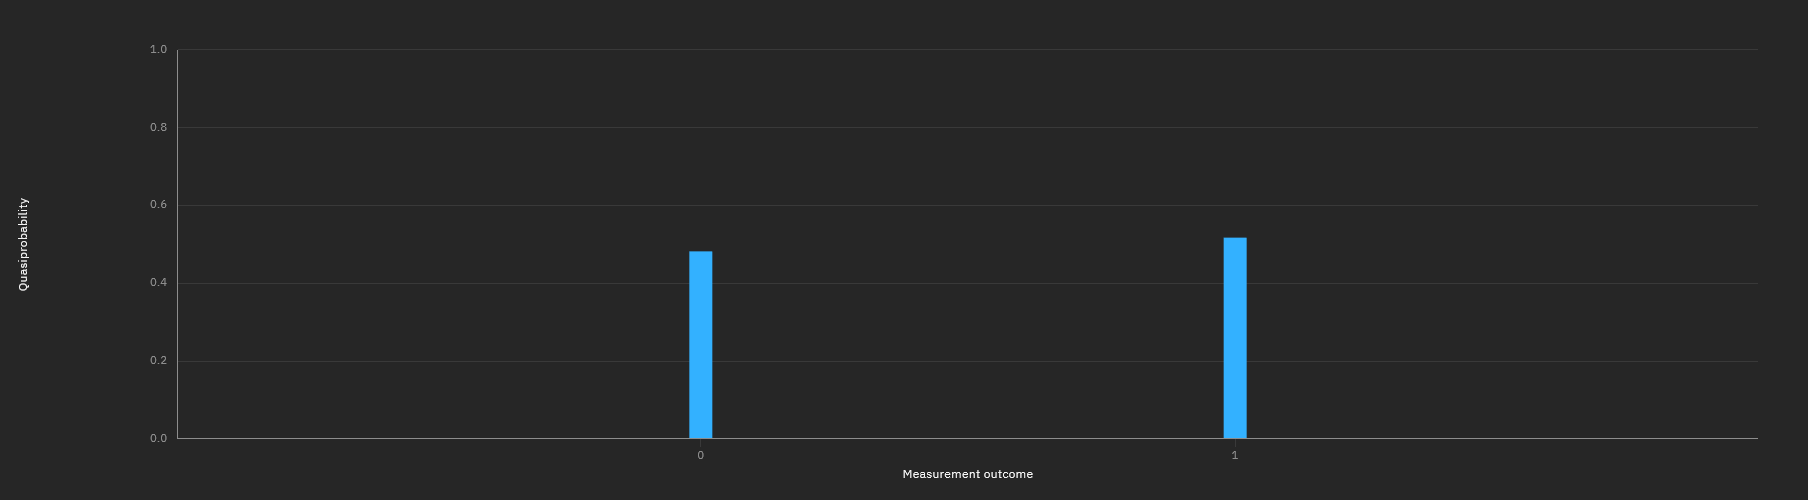
\includegraphics[scale=0.27]{a.png}
    \caption{The results of the measurement of the circuit (a) after 1024 shots.}
\end{figure}

\paragraph*{\text{b)}}

The double Hadamard gates will cancel each other out, so the qubit remains in the $|0⟩$ state. The measurement should result in $|0⟩$ with $100\%$ probability. After testing the circuit with 1024 shots, the results are very close as expected with $ 99.7\%$.

\begin{figure}[H]
    \centering
    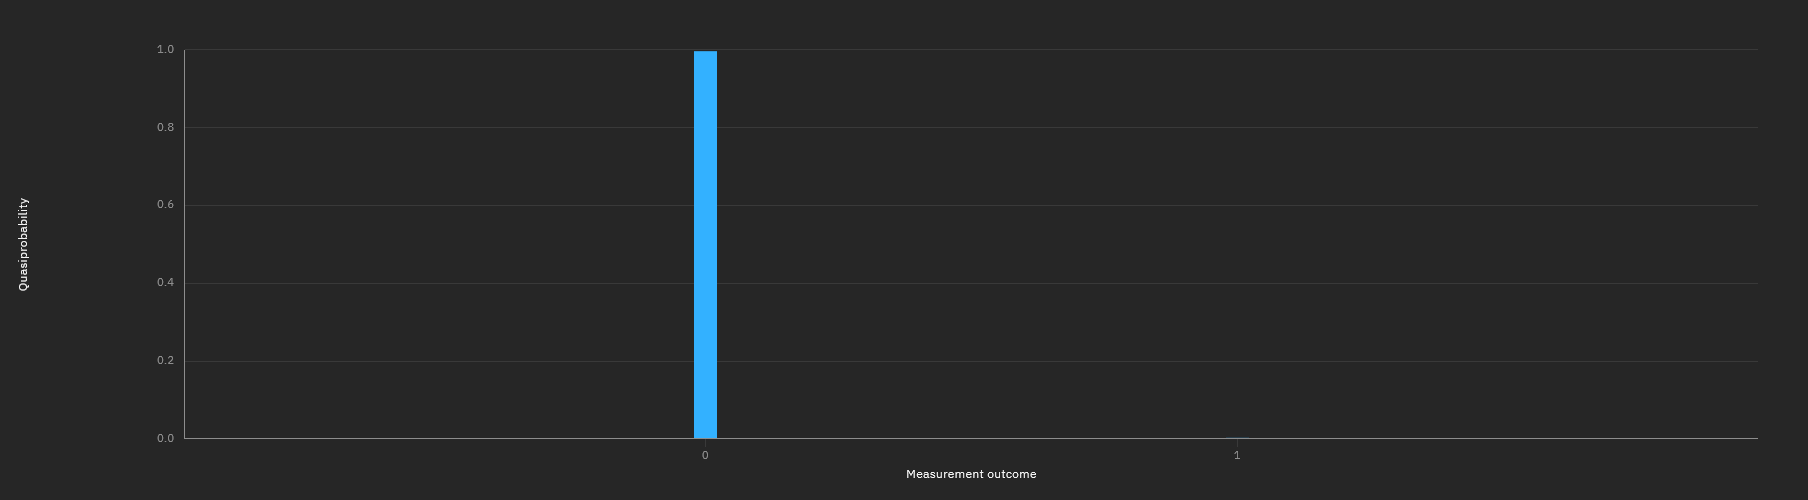
\includegraphics[scale=0.27]{b.png}
    \caption{The results of the measurement of the circuit (b) after 1024 shots.}
\end{figure}

\newpage

\paragraph*{\text{c)}}

The Hadamard gate puts the first qubit into a superposition, and the CNOT gate entangles the two qubits. The measurement of the first qubit will collapse it to either $|0⟩$ or $|1⟩$ with equal probability. If the first qubit is measured as $|0⟩$, the second qubit will also be $|0⟩$ due to the CNOT gate. If the first qubit is measured as $|1⟩$, the second qubit will be flipped to $|1⟩$. Thus, there should be a $50\%$ chance of measuring $|00⟩$ and a $50\%$ chance of measuring $|11⟩$, and it is actually the Bell state. After testing the circuit with 1024 shots, the results are close to the expected, $50.6\%$ for $|00⟩$ and $50.2\%$ for $|11⟩$ and some negative results for the others as $-0.5\%$ and $-0.3\%$.

\begin{figure}[H]
    \centering
    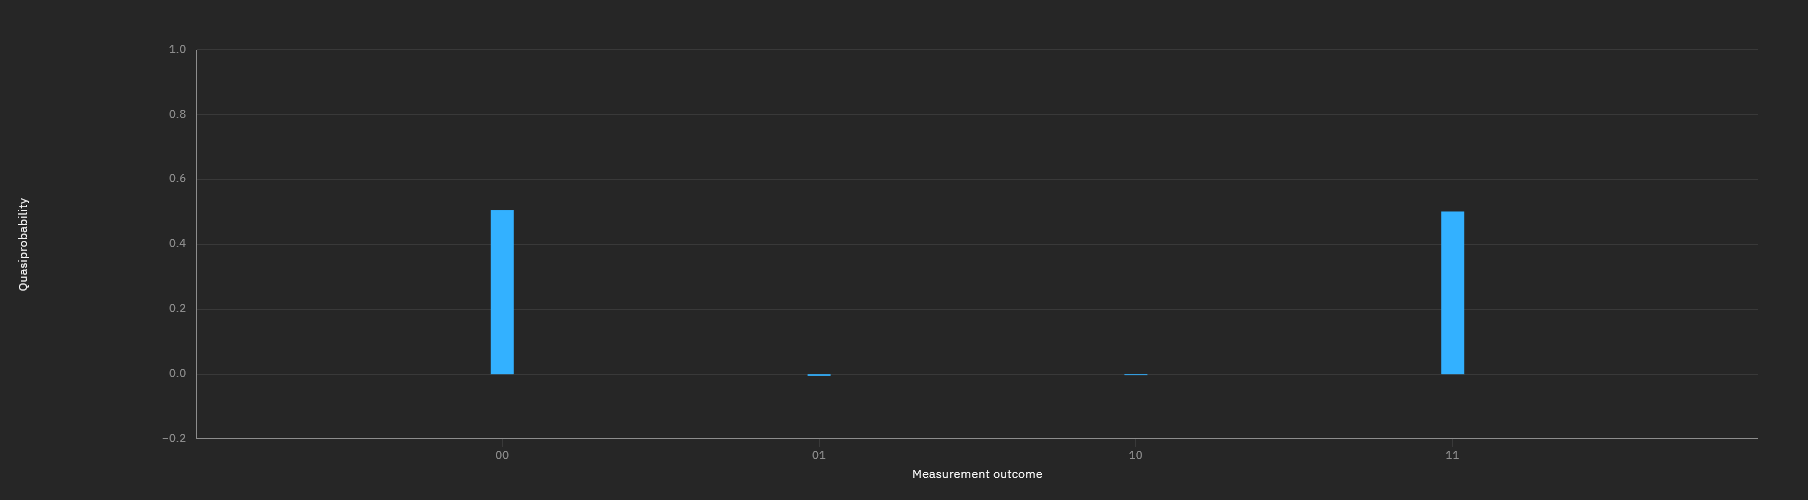
\includegraphics[scale=0.27]{c.png}
    \caption{The results of the measurement of the circuit (c) after 1024 shots.}
\end{figure}

\paragraph*{\text{d)}}

The Hadamard (H) gate on the first qubit puts it into a superposition of $|0⟩$ and $|1⟩$. The CNOT gate then creates entanglement between the first and second qubit, with the first qubit as the control. If the control qubit is $|0⟩$, the target qubit (second qubit) remains at $|0⟩$; if the control qubit is $|1⟩$, the target qubit flips to $|1⟩$. Another Hadamard gate on the first qubit before measurement can reintroduce interference between the paths that lead to $|00⟩$ and $|11⟩$, giving equal probabilities to $|00⟩$ and $|11⟩$, as well as creating a non-zero probability for $|01⟩$ and $|10⟩$ due to the superposition being re-established after CNOT gate, so the expected probabilities are equal on each state with $25\%$. The results are close but with higher errors than the previous ones, $24\%$, $28.3\%$, $18.9\%$ and $28.9\%$ from 00 to 11.    

\begin{figure}[H]
    \centering
    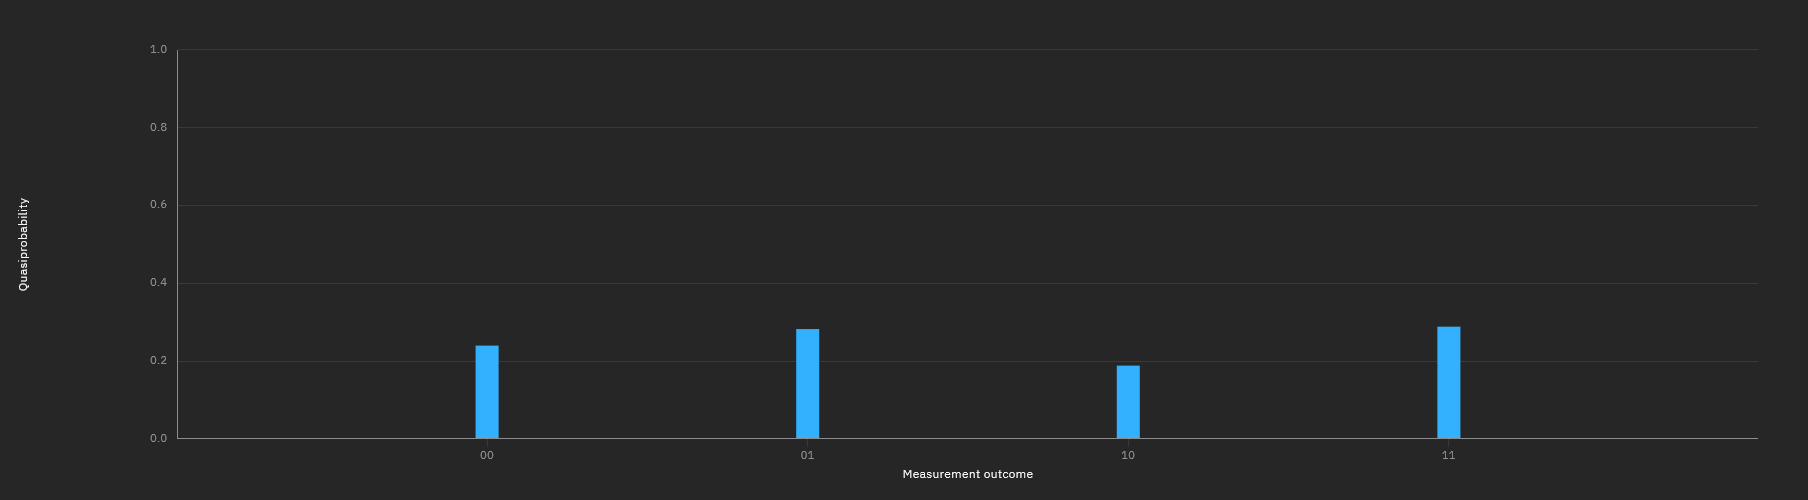
\includegraphics[scale=0.27]{d.png}
    \caption{The results of the measurement of the circuit (d) after 1024 shots.}
\end{figure}

\newpage

\paragraph*{\text{e)}}

This circuit is similar to the previous one, this time the second qubit is a control qubit of another CNOT gate, the expected chances of states were equal. This time there is a third qubit, which is being controlled by the second, will only flip if the second qubit is $|1⟩$ after the first measurement. The result is that the probabilities are spread among $|000⟩$, $|001⟩$, $|110⟩$, and $|111⟩$, as the entanglement and superposition distribute the probabilities. The measurement results are close to the expected, but there are some errors on these states, $23.8\%$, $27.7\%$, $17.2\%$ and $32\%$ respectively.

\begin{figure}[H]
    \centering
    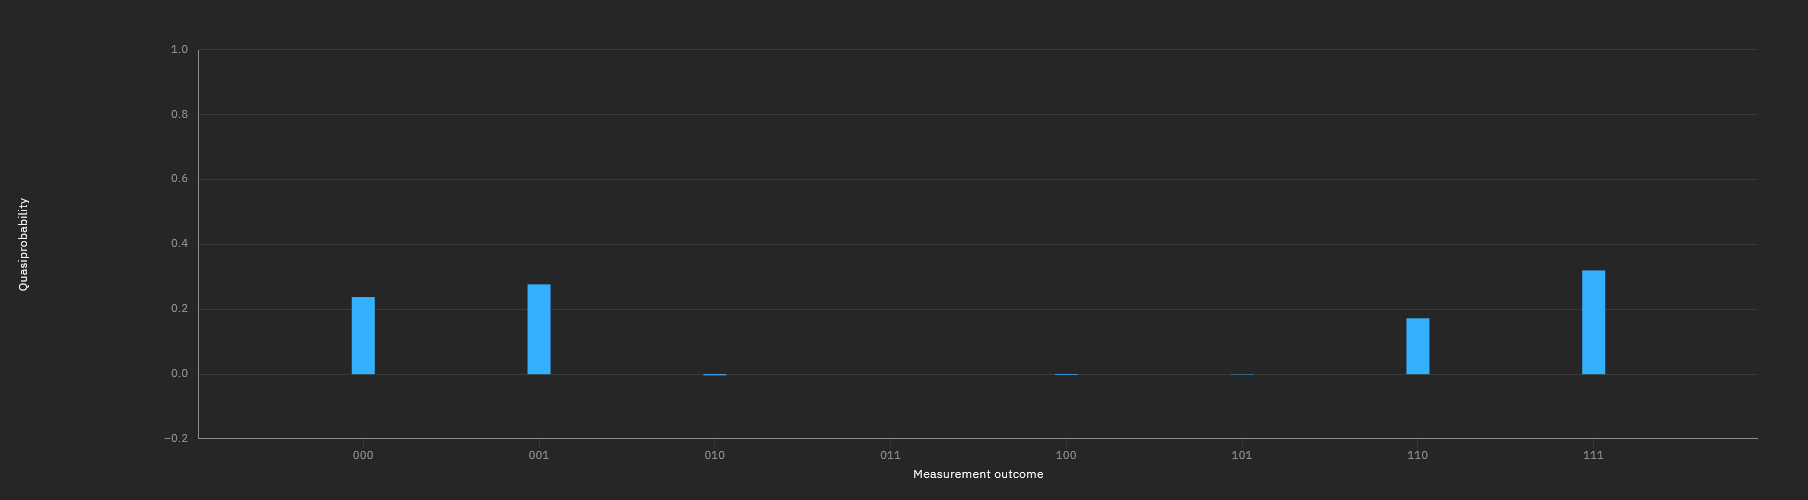
\includegraphics[scale=0.27]{e.png}
    \caption{The results of the measurement of the circuit (e) after 1024 shots.}
\end{figure}

\paragraph*{\text{f)}}

The Hadamard gate on the first qubit creates a superposition, and the subsequent CNOT gates entangle the first and second qubits, and then the second and third qubits. The additional Hadamard gate on the second qubit before the CNOT with the third qubit adds complexity to the entanglement. This can lead to a situation where all possible states have an almost equal probability because of the multiple layers of superposition and entanglement created by the sequence of gates. The measurement gives a similar result with a high error on some of the states, $12.3\%$, $13.3\%$, $16\%$, $10.6\%$, $12.4\%$, $11.9\%$, $10.7\%$ and $12.8\%$ from 000 to 111.

\begin{figure}[H]
    \centering
    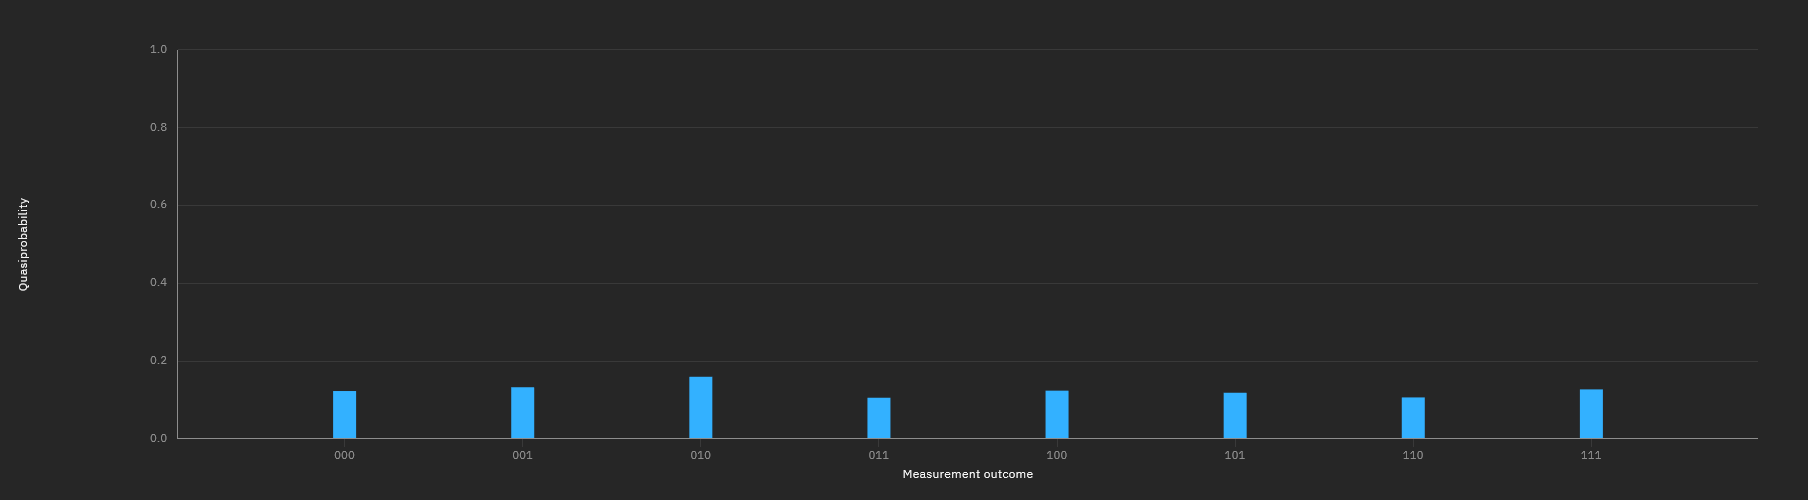
\includegraphics[scale=0.27]{f.png}
    \caption{The results of the measurement of the circuit (f) after 1024 shots.}
\end{figure}




\end{document}
